\section{Methodology}

\begin{figure*}[t]
  \centering
  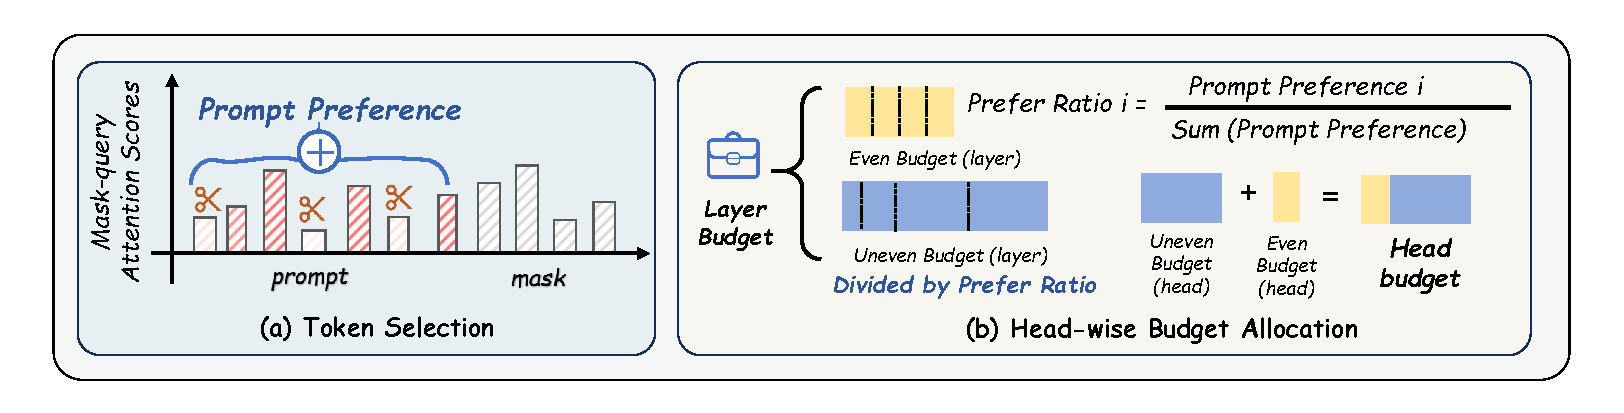
\includegraphics[width=1.0\linewidth]{figure/pipe_final.pdf}
  \caption{\textbf{The \mymethod{} pipeline.} We use Mask Voting to assess token importance, then apply adaptive budget allocation where layers and heads receive budgets by boundary awareness and prompt preference. Tokens are evicted based on their importance under the given budget.}
  \label{fig:pipline}
\end{figure*}



\subsection{Preliminaries}

\noindent \textbf{Inference of Diffusion Large Language Models.}
Diffusion language models (dLLMs) generate text through an iterative unmasking process over T discrete decoding steps, progressively refining a fully masked sequence into the final output.
We first define the token vocabulary as $\mathcal{T}$, which includes a special mask token $\texttt{[MASK]} \in \mathcal{T}$.  
For a given prompt $c=(c_1,\dots,c_M)$, the initial input state is 
\begin{equation}
x^{(T)} = [c_1, \dots, c_M, \underbrace{\texttt{[MASK]}, \dots, \texttt{[MASK]}}_{L}]
\end{equation}
where L is the pre-specified target response length.

Unlike ARMs, which extend the sequence token by token, diffusion language models (dLLMs) refine the entire sequence in parallel at every step. This sequence includes the prompt, already decoded tokens, and remaining \texttt{[MASK]} tokens. \\
At each step t, the model $f_\phi$ takes the current state $x 
^{(t)}$ and predicts a probability distribution over the vocabulary for every masked position, resulting in $y = \{y_i \mid i \in M^{(t)}\}$, the set of candidate tokens for all masked locations:
\begin{equation}
P_\phi(y \mid x^{(t)}) = f_\phi(x^{(t)})
\end{equation}
and remasking policy $\mathcal{R}$ decides which tokens to decode and which to keep masked in the next step.
\begin{equation}
x^{(t-1)} = \mathcal{R}\big(x^{(t)}, P_\phi(y \mid x^{(t)})\big)
\end{equation}
The process continues until step t=0, at which point all \texttt{[MASK]} tokens have been replaced to yield the final sequence. 
This design enables parallel multi-token prediction but at the expense of substantial computational and memory costs. 

\noindent \textbf{Caching in Diffusion Large Language Models }
Given the initial input $x^{(T)}$ composed of a prompt of length $M$ and $L$ masked positions, we denote the prompt and response token sets as $\mathcal{P}=\{1\!:\!M\}$ and $\mathcal{R}=\{M\!+\!1\!:\!M\!+\!L\}$, respectively. We index layers by $\ell=1,\ldots,D$. At denoising step $t$, for layer $\ell$ and position $i$, we define the cacheable feature bundle 
\begin{equation}
\mathrm{Feat}_{\ell}^{(t)}(i)
= \{ K_{\ell,i}^{(t)}, V_{\ell,i}^{(t)}, \mathrm{Attn}_{\ell,i}^{(t)}, \mathrm{FFN}_{\ell,i}^{(t)} \}
\end{equation}
and denote the cache entry by $\mathcal{C}_{\ell}^{(t)}(i)$. And each layer forward pass computes:
\begin{equation}
  h_{\ell}^{(t)} 
  = \mathrm{Attn}_{\ell}\!\bigl(Q_{\ell}^{(t)}, K_{\ell}^{(t)}, V_{\ell}^{(t)}\bigr)
  + \mathrm{FFN}_{\ell}
  \label{eq:layer_forward}
\end{equation}
Unlike autoregressive models, where causal attention allows past KV states to be directly reused, diffusion LLMs employ bidirectional attention over both prompt and masked positions, which prevents the reuse of intermediate states. Because this operation is repeated for every step and every token, it introduces substantial computational redundancy. Empirically, however,the feature bundles $\mathrm{Feat}_{\ell}^{(t)}(i)$ exhibit strong similarity across adjacent steps, suggesting opportunities for caching~\citep{liu2025dllm,wu2025fast,ma2025dkv,hu2025accelerating}.

At each step $t$, if $i \in \mathcal{S}^{(t)}$, we refresh 
$\mathcal{C}_{\ell}^{(t)}(i)=\mathrm{Feat}_{\ell}^{(t)}(i)$;  
otherwise, we reuse $\mathcal{C}_{\ell}^{(t-1)}(i)$. The definition of $\mathcal{S}^{(t)}$ differs by token type.  

\paragraph{Prompt tokens.}
For prompt tokens ($i\in\mathcal{P}$), we refresh them only every $T_{p}$ steps, 
i.e., $\mathcal{S}_{\mathcal{P}}^{(t)}=\{\,i\in\mathcal{P}\mid t\bmod T_{p}=0\,\}$; 
between refreshes, their cached features remain fixed.

\paragraph{Response tokens.}
For response tokens, we define two candidate refresh sets: 
$\mathcal{S}_{\mathrm{period}}^{(t)}=\{\,i\in\mathcal{R}\mid t\bmod T_r=0\,\}$ 
representing tokens refreshed periodically every $T_r$ steps, and 
$\mathcal{S}_{\mathrm{shift}}^{(t)}=\{\,i\in\mathcal{R}\mid 
\cos(V_{\ell,i}^{(t)},V_{\ell,i}^{(t-1)})<\delta\,\}$ 
representing tokens whose feature vectors vary significantly between consecutive steps.
The overall refresh set is given by 
$\mathcal{S}_{\mathcal{R}}^{(t)}=
\mathcal{S}_{\mathrm{period}}^{(t)}\cup
\mathcal{S}_{\mathrm{shift}}^{(t)}$.

\subsection{Observations}
Our hierarchical compression strategy stems from a top-down analysis of the dLLM's attention architecture, which revealed optimization opportunities at the layer, head, and token levels.

\paragraph{Layer-Level.}
Our analysis begins at the highest architectural level: the importance of each Transformer layer. We quantify this importance by measuring each layer's representational transformation, which we formalize as an \textbf{importance score} (see Section~\ref{sec: method}). Our analysis of these scores reveals two critical phenomena, both visualized in Fig.~\ref{fig:attention_map}~(b): a distinct \textbf{bimodal importance profile} and strong \textbf{cross-sample consistency}.

The bimodal profile is visually evident as the boundary layers (the first and last columns) consistently exhibit lighter colors than the middle layers, signifying lower cosine similarity and thus higher importance. The cross-sample consistency is demonstrated by the vertical uniformity of this pattern across all samples, indicating that this importance hierarchy is remarkably stable.
These two findings form the cornerstone of our allocation strategy. The bimodal profile dictates the need for a non-uniform, group-based allocation, while the cross-sample consistency validates the feasibility of a static, offline approach.

\paragraph{Head-Level.}
Building on our layer-level findings, we next analyzed the behavior of individual attention heads. Our analysis reveals a significant functional heterogeneity, as different heads exhibit widely varying degrees of dependency on the prompt context. The examples in Fig.~\ref{fig:attention_map}~(c) clearly illustrate this. The head we term the \textbf{Information Head} is highly dependent on the prompt to perform long-range information retrieval. Conversely, the \textbf{Structure Head} shows a low dependency on the prompt, as its primary role is to plan the discourse structure by organizing the syntactic framework. This observed variation is the direct motivation for our next strategy: a fine-grained, head-wise budget allocation, weighted according to each head's reliance on the prompt context.

\paragraph{Token-Level.}
Finally, after allocating budgets to layers and heads, a universal criterion is needed to select the specific tokens to retain. Our analysis of token-level attention patterns reveals this criterion. A crucial dichotomy emerges (see Fig.~\ref{fig:attention_map} (a)): non-mask tokens (\textit{i.e.}\, the prompt and already-decoded tokens) exhibit a strong \textbf{locality bias}, serving to encode their own context. In stark contrast, attention from mask queries is \textbf{highly sparse and long-range}, functioning as a task-driven information retrieval mechanism. Critically, this sparse attention is also \textbf{remarkably consistent} across all generation steps. This provides the final piece of our framework: the attention from mask queries serves as the definitive and stable signal for token importance, applicable to any head.

\subsection{The \emph{MaskKV} Framework}
\label{sec: method}
Based on our empirical findings, we propose \emph{MaskKV}, a framework that reframes KV cache pruning as a two-stage process: first, it establishes a universal importance ranking for all tokens, and second, it applies a hierarchical budget to this ranking to perform eviction.

\paragraph{Stage 1: Universal Token Importance Ranking.}

We observe that, unlike prompt queries which exhibit local bias, mask queries perform sparse long‑range retrieval with strong cross‑step consistency, making them reliable indicators of token importance. This aligns with our theoretical proof (Appendix~\ref{the primacy of mask attention}) that mask‑guided attention provides the most direct signal for the generative task.
Consequently, we propose \textbf{Mask-Voting}, a one-shot method that leverages the reliable, task-aligned signal from mask queries at the initial inference step.

We first compute the attention score matrix $A$ from all mask queries ($Q_{mask}$) to all keys ($K_{full}$):
\begin{equation}
    A = \text{softmax}_{\text{row}}\left(\frac{Q_{mask} K_{full}^T}{\sqrt{d_k}}\right)
\end{equation}
From this matrix, we derive an importance score vector $I \in \mathbb{R}^{n_p}$ for the prompt tokens by aggregating the scores each key receives:
\begin{equation}
    I_j = \sum_{i=1}^{n_m} A_{ij} \quad \text{for } j \in \{1, \dots, n_p\}
\end{equation}
The output of this stage is the vector $I$, which provides a universal, budget-agnostic importance ranking of all prompt tokens.

\paragraph{Stage 2: Hierarchical Budgeted Eviction.}
The second stage determines the fine-grained, per-head eviction budget $k_{l,h}$ using a top-down allocation policy. This process systematically distributes the total prompt budget, $k_p$, across the model's layers and then its heads, guided by data-driven importance metrics.

At the \textbf{layer level}, we allocate the total budget $k_p$ based on layer importance. We quantify this importance using a score, $I^{(l)}$, that measures the representational transformation performed by each layer. A larger transformation signifies higher importance. Inspired by prior work~\citep{wang2024squeezeattention, he2024matters}, we define it as:
\begin{equation}
\label{eq:layer_importance_metric}
    I^{(l)} = 1 - \frac{1}{n} \sum_{i=1}^{n} \text{cos\_sim}\left(h_{in, i}^{(l)}, h_{out, i}^{(l)}\right)
\end{equation}
where $h_{in, i}^{(l)}$ and $h_{out, i}^{(l)}$ are the input and output hidden states of the attention sub-layer for the $i$-th token.

With the layer importance score $I^{(l)}$ defined, we now detail our hybrid allocation strategy. The total budget $k_p$ is first partitioned into a uniform base component and an importance-driven component. The per-layer base budget, $k_{\text{base}}$, is set by a hyperparameter $\beta \in [0,1]$:
\begin{align}
    k_{\text{base}} &= \left\lfloor \frac{\beta \cdot k_p}{L} \right\rfloor \\
    k_{\text{imp}} &= k_p - L \cdot k_{\text{base}}
\end{align}
where $k_{\text{imp}}$ is the total remaining budget to be allocated based on importance. 

Next, we distribute $k_{\text{imp}}$ to the boundary ($S_{\text{bound}}$) and middle ($S_{\text{mid}}$) layer groups, proportional to their aggregated importance scores ($I_g = \sum_{l \in S_g} I^{(l)}$). This yields the \textit{total group budgets}, denoted $k_{\text{group},B}$ and $k_{\text{group},M}$:
\begin{align}
\label{eq:group_budget_allocation}
k_{\text{group},B} &= k_{\text{imp}} \cdot \frac{I_B}{I_B + I_M} \\
k_{\text{group},M} &= k_{\text{imp}} - k_{\text{group},B}
\end{align}
Finally, the budget for any given layer, $k_l$, is the sum of its base budget and an equal share of its group's importance-driven budget:
\begin{equation}
\label{eq:final_layer_budget}
    k_l = k_{\text{base}} + 
    \begin{cases} 
        \left\lfloor \dfrac{k_{\text{group},B}}{|S_{\text{bound}}|} \right\rfloor & \text{if } l \in S_{\text{bound}} \\
        \left\lfloor \dfrac{k_{\text{group},M}}{|S_{\text{mid}}|} \right\rfloor & \text{if } l \in S_{\text{mid}} 
    \end{cases}
\end{equation}

An ``online'' implementation of this algorithm is fundamentally flawed for reducing peak memory. Budget allocation requires scores from all layers, which necessitates a full forward pass with the entire, uncompressed KV cache stored. Eviction could only occur \textit{after} the peak memory has already been reached. Therefore, leveraging our finding of \textbf{cross-sample consistency}, we adopt an \textbf{offline} paradigm. By pre-computing a importance profile on a calibration set, we can determine all budgets \textit{a priori}, enabling immediate layer-by-layer eviction that effectively reduces the peak memory footprint.

At the \textbf{head level}, the per-layer budget $k_l$ is distributed among its $N_h$ heads. This allocation is guided by each head's \textbf{Prompt Preference}, $P_h^{(l)}$, which quantifies its dependency on the prompt:
\begin{equation}
\label{eq:prompt_preference_metric}
    P_h^{(l)} = \frac{S_{m \to p}^{(l,h)}}{S_{m \to p}^{(l,h)} + S_{m \to m}^{(l,h)}}
\end{equation}
where $S_{m \to p}^{(l,h)}$ and $S_{m \to m}^{(l,h)}$ are the sums of mask-to-prompt and mask-to-mask attention, respectively.

The final, fine-grained budget for each head, $k_{l,h}$, is calculated via a hybrid strategy controlled by a hyperparameter $\alpha \in [0,1]$. This strategy combines a fixed base allocation with a proportional allocation based on preference into a single formula:
\begin{equation}
\label{eq:final_head_budget}
    k_{l,h} = \left\lfloor \alpha \cdot k_l + (1-\alpha) \cdot N_h \cdot k_l \cdot \hat{P}_h^{(l)} \right\rfloor
\end{equation}
where $\hat{P}_h^{(l)} = P_h^{(l)} / \sum_{j=1}^{N_h} P_j^{(l)}$ is the normalized Prompt Preference score.

Finally, with the universal importance ranking $I$ from Stage 1 and the specific per-head budget $k_{l,h}$ from Stage 2, the eviction is performed by selecting the top-k tokens:
\begin{equation}
    S_{\text{keep}} = \operatorname{arg\,topk}(I, k_{l,h})
\end{equation}







